%!TEX root = ../main.tex
We want to use this theory to justify more formally the method we introduced.

Let's start under the hypothesis that our model class is rich enough to describe our system.
\begin{equation*}
S\in \Mc \quad \left(\text{i.e. }\exists\,\theta _{0} \in \Theta :S\equiv y(t) =\frac{B\left(z,\theta _{0}\right)}{A\left(z,\theta _{0}\right)} u(t-d) +\frac{C\left(z,\theta _{0}\right)}{A\left(z,\theta _{0}\right)} e(t),\, e(t) \sim \WN(0,\lambda ^{2})\right)
\end{equation*}
Our model is not just a model, but the true system through which $ y(t)$ is generated.

The expression of the asymptotic cost function is:
\begin{align*}
	\bar{J}(\theta) & =\E\left[ \varepsilon (t,\theta)^{2}\right] \\
	& = \E\left[(y(t) -\hat{y}(t\mid t-1,\theta))^{2}\right] \\
	& = \E\left[\left(y(t) \pm \hat{y}\left(t\mid t-1,\theta _{0}\right) -\hat{y}(t\mid t-1,\theta)\right)^{2}\right] \\
	& = \E\bigg[(\underbrace{
			y(t) -\hat{y}\left(t\mid t-1,\theta_{0}\right)
		}_{
			\substack{=e_{0}(t) \\ \text{generated by $S=\Mc(\theta_{0})$} \\ \text{opt. predictor}}
		}
		+ \hat{y}\left(t\mid t-1,\theta _{0}\right) -\hat{y}(t\mid t-1,\theta))^{2}\bigg] \\
	& = \E\bigg[(e_{0}(t) + \underbrace{
			\hat{y}\left(t\mid t-1,\theta _{0}\right) -\hat{y}(t\mid t-1,\theta
		}_{
			\substack{\text{$\hat{y}$ linear functions} \\ \text{of $y(t-1),y(t-2),\ldots$} \\ \text{uncorrelated with $e_{0}(t)$}}
		}
		))^{2}\bigg] \\
	& = \E\left[ e_{0}(t)^{2}\right] +\E\left[\left(\hat{y}\left(t\mid t-1,\theta _{0}\right) -\hat{y}(t\mid t-1,\theta)\right)^{2}\right] \\
	& = \underbrace{\lambda _{0}^{2}}_{\text{const.}} +\underbrace{\E\left[\left(\hat{y}\left(t\mid t-1,\theta _{0}\right) -\hat{y}(t\mid t-1,\theta)\right)^{2}\right]}_{\geq 0,\ =0\text{ if } \theta =\theta _{0}}
\end{align*}

So that
\begin{equation*}
\bar{J}\left(\theta _{0}\right) = \lambda _{0}^{2} \leq \bar{J}(\theta)\  \forall \theta \quad\Longrightarrow\quad \theta _{0} \text{ is a minimum of } \bar{J}(\theta)
\end{equation*}
Using \gls{pem} asymptotic theory
\begin{equation*}
\text{distance}[\hat{\theta}_{N}(s), \Delta]\xrightarrow{N\to\infty} 0 \quad \text{with }\theta_{0} \in \Delta 
\end{equation*}
If $ \Delta =\left\{\theta _{0}\right\}$ is a singleton (i.e. $ \bar{J}$ has unique minimum) then:
\[
	\boxed{
		\begin{aligned}
			\hat{\theta }_{N} & \xrightarrow{N\rightarrow \infty} \theta _{0}\\
			\Mc(\hat{\theta }_{N}) & \xrightarrow{N\rightarrow \infty} S
		\end{aligned}
	}
\]
Thus, the \gls{pem} identification is \textbf{asymptotically consistent}: if $ \Mc$ is rich enough and the number of collected data is big enough, \gls{pem} identification provides a good description of $ S$.



\section{Model order selection}

The identification of model consists of 4 steps:
\begin{enumerate}
\item data collection;
\item choice of $ \Mc$;
\item optimal model selection\footnote{\gls{pem}: $ \hat{\theta }_{N} =\underset{\theta \in \Theta }{\argmin} J_{N}(\theta)$};
\item model validation\footnote{evaluate the performance of $\Mc(\hat{\theta }_{N})$}.
\end{enumerate}

The process is not linear: it is common to loop from model validation to another choice of $ \Mc$ (if the model is not satisfactory) or even to data collection.

An important choice for $ \Mc$ is the model order selection. Given an ARMAX model (black-box case):
\begin{gather*}
\begin{aligned}
y(t)  & =\frac{B(z,\theta)}{A(z,\theta)} u(t-d) +\frac{1}{A(z,\theta)} e(t) & e(t) \sim \WN (0,\lambda ^{2})\\
A(z,\theta)  & =1-a_{1} z^{-1} -\cdots -a_{m} z^{-m} & \\
B(z,\theta) & =b_{0} +b_{1} z^{-1} +\cdots +b_{p} z^{-p} & \\
C(z,\theta) & =1+c_{1} z^{-1} +\cdots +c_{n} z^{-n} & 
\end{aligned}\\
\end{gather*}
The model order is: $ (m,p,n)$, the delay $ d$ between $ I/O$ is neglected as it can be easily retrieved from data.

Notice that some trivial choices for model selection change the structure of the model:
\begin{equation*}
\begin{cases}
n=0 & \text{ARX}\\
n=0,p=0 & \text{AR}\\
n\neq 0,p=0 & \text{ARMA}
\end{cases}
\end{equation*}
However, we will deal with the case where the structure is fixed ($ n,m,p\neq 0\Longrightarrow$ ARMAX) and we just want to select a proper number. To keep the notation simple we will focus on one hyper-parameter ($ m=n=p$) without loss of generalization.

A naive idea is to use $ J_{N}$ as an indicator for model quality, selecting a maximum value for the model order. Cycling for $ m=1:\overline{m}$, where $\overline{m}$ is the maximum model order we allow for:

\boxedText{
	$\mathtt{For }\ m=1:\overline{m}$
	\begin{gather*}
		\Mc^{m} =\text{ARMAX}(m) =\left\{\Mc(\theta) ,\theta \in \Theta ^{m}\right\}\\
		\hat{\theta }_{N}^{m} =\underset{\theta \in \Theta ^{m}}{\argmin}\frac{1}{N}\sum _{i=1}^{N}(y(i) -\hat{y}(i\mid i-1,\theta))^{2}
	\end{gather*}
	$\mathtt{END}$
}

At the end of the cycle we select:
\begin{equation*}
\hat{\theta }_{N} =\hat{\theta }_{N}^{m} \text{ with lowest } J_{N}(\hat{\theta }_{N}^{m})
\end{equation*}
\begin{obs}
	This naive idea does NOT work in practice: $ J_{N}(\hat{\theta }_{N}^{m})$ is always decreasing with $ m$, so that the highest possible order is selected. As $m$ increases, the model runs in the problem of over-fitting: it's perfectly good for describing the data collected but it does not generalizes to new data. The model has overall a bad predictive performance on new data.
\end{obs}
\begin{figure}[htpb]
    \centering
    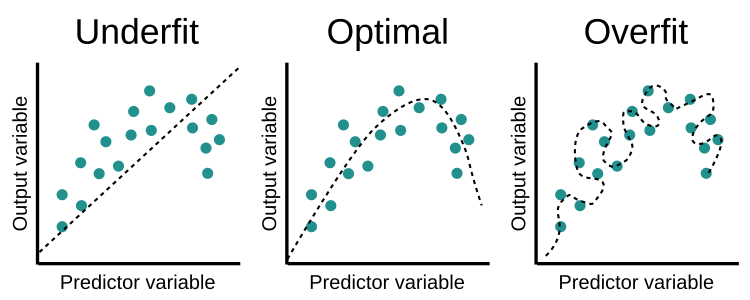
\includegraphics[width=0.5\linewidth]{over-under-fit}
    \caption{Meaning of underfitting and overfitting.}
\end{figure}
\FloatBarrier
A very simple but powerful idea to solve the problem is to perform \textbf{cross validation}.

Cross validation consists in evaluating the performance of an identified model on new data: the dataset is divided in two parts, using the first (\textbf{training dataset}) for selecting the parameters and the second (\textbf{validation dataset}) for cross validation.

The for-loop becomes:

\boxedText{
	$\mathtt{For } \ m=1:\overline{m}$
	\begin{gather*}
		\Mc^{m} =\text{ARMAX}(m) =\left\{\Mc(\theta) ,\theta \in \Theta ^{m}\right\}\\
		\hat{\theta }_{T}^{m} =\underset{\theta \in \Theta ^{m}}{\argmin} J_{T}(\theta) =\underset{\theta \in \Theta ^{m}}{\argmin}\frac{1}{M}\sum _{i=1}^{M}(y(i) -\hat{y}(i\mid i-1,\theta))^{2}\\
		J_{V}(\hat{\theta }_{T}^{m}) =\frac{1}{N-M}\sum _{i=M+1}^{N}\left(y(i) -\hat{y}\left(i\mid i-1,\hat{\theta }_{T}^{m}\right)\right)^{2}
	\end{gather*}
	$\mathtt{END}$
}

Where $ J_{V}$ is the performance of the model obtained from the training set evaluated on the validation dataset. Then we select
\begin{equation*}
m^{\star} =\underset{m}{\argmin} J_{V}(\hat{\theta }_{T}^{m}) ,\hat{\theta }_{N} =\hat{\theta }_{T}^{m^{\star}}
\end{equation*}

\fg{0.6}{cross-validation}
The drawback of cross-validation is that the dataset has to be split: less information is used to tune the model and data collection can be expensive.


\subsection{Alternative approach: direct model order penalization}
The structure is similar, we run a cycle up to a maximum model order

\boxedText{
	$\mathtt{For } \ m=1:\overline{m}$
	\begin{gather*}
		\Mc^{m} =\text{ARMAX}(m) =\left\{\Mc(\theta) ,\theta \in \Theta ^{m}\right\} \\
		\hat{\theta }_{N}^{m}  =\underset{\theta }{\argmin}\frac{1}{N}\sum _{i=1}^{N}(y(i) -\hat{y}(i\mid i-1,\theta))^{2}\\
		V(m) =V(m,J_{N}(\hat{\theta }_{N}^{m})),\forall m
	\end{gather*}
	$\mathtt{END}$
}

All data is used to tune the model.

Then we select
\begin{equation*}
m^{\star} =\underset{m}{\argmin} V(m) ,\hat{\theta }_{N} =\hat{\theta }_{T}^{m^{\star}}
\end{equation*}
Some common choice are
\begin{align*}
\text{FPE} & =\text{Final Prediction Error} & \text{(probability)}\\
\text{AIC} & =\text{Akaike's Identification Criterion} & \text{(statistics)}\\
\text{MDL} & =\text{Minimum Description Length} & \text{(information theory)}
\end{align*}
\begin{equation*}
	\begin{array}{rcc}
		\text{FPE}(m) = & \frac{N+m}{N-m}          &  \cdot J_{N}(\hat{\theta }_{N}^{m})\\
		\text{AIC}(m) = & 2\frac{m}{N}             &  +\ln(J_{N}(\hat{\theta }_{N}^{m}))\\
		\text{MDL}(m) = & \ln(N)\frac{m}{N}        &  +\ln(J_{N}(\hat{\theta }_{N}^{m}))\\
		                & \text{increasing with }m &  \text{decreasing with }m
	\end{array}
\end{equation*}
In fact, FPE and AIC are approximately equivalent:
\begin{align*}
\ln(\text{FPE}) & =\ln\left(\frac{N+m}{N-m} J_{N}(\hat{\theta }_{N}^{m})\right) \\
 & =\ln\left(\frac{1+\frac{m}{N}}{1-\frac{m}{N}} J_{N}(\hat{\theta }_{N}^{m})\right) \\
 & =\ln\left(1+\frac{m}{N}\right) -\ln\left(1-\frac{m}{N}\right) +\ln(J_{N}(\hat{\theta }_{N}^{m})) \quad m\ll N, \frac{m}{N} \approx 0\\
 & \approx \frac{m}{N} -\left(-\frac{m}{N}\right) +\ln(J_{N}(\hat{\theta }_{N}^{m})) \\
 & =2\frac{m}{N} +\ln(J_{N}(\hat{\theta }_{N}^{m})) = \text{AIC} & 
\end{align*}
MDL is equal to AIC with 2 replaced by $ \ln(N)$. Since typically $ \ln(N)  >2$ (i.e. dataset has more than 8 data points) MDL penalizes model order more than AIC and FPE.


% esercitazione 10

\section{Estimation of mean, covariance and spectrum}

\subsection{Mean}

We use the sample mean:
\[
	\boxed{\hat{m}_{N}=\frac{1}{N}\sum_{t=1}^{N} y(t)} 
\]
\begin{itemize}
	\item it is \textbf{correct}: $\E[\hat{m}_{N}]=m=\E[y(t)]$;
	\item if $\gamma _{y}(\tau )\xrightarrow{|\tau|\to\infty} 0$ then it is \textbf{consistent}: $\E[(\hat{m}_{N}-m)^2]\xrightarrow{N\to\infty} 0$.
\end{itemize}

\subsection{Covariance}

We estimate it through
\[
	\boxed{\hat{\gamma}_{y}(\tau) = \frac{1}{N-|\tau|} \sum_{t=1}^{N-|\tau|} y(t)\cdot y(t+|\tau|), \qquad |\tau|\leq N-1}
\]
Increasing $|\tau|$, the number of terms to add is lower and lower. It works well when $|\tau|$ is smaller than $N$ (generally $N\geq 50$ and $|\tau|\leq N/4$).
\begin{itemize}
	\item it is \textbf{correct}: $\E[\hat{\gamma}_{y}(\tau)]=\gamma_{y}(\tau)$;
	\item if $\gamma _{y}(\tau )\xrightarrow{|\tau|\to\infty} 0$ then it is \textbf{consistent}.
\end{itemize}

Usually, another estimator for the covariance function is used:
\[
	\boxed{\hat{\gamma}_{y}'(\tau) = \frac{1}{N} \sum_{t=1}^{N-|\tau|} y(t)\cdot y(t+|\tau|), \qquad |\tau|\leq N-1}
\]
\begin{itemize}
	\item it is \textbf{not correct}: $\E[\hat{\gamma}_{y}'(\tau)]=\frac{N-|\tau|}{N}\gamma _{y}(\tau)$, but it is \textbf{asymptotically correct} (it becomes so for $N\to\infty$);
	\item if $\gamma _{y}(\tau )\xrightarrow{|\tau|\to\infty} 0$ then it is \textbf{consistent};
	\item leads to simpler methods for spectrum estimation.
\end{itemize}

\subsection{Spectrum}

We define two estimators:
\[
	\boxed{\hat{\Gamma}_{y}(\omega) = \sum_{\tau = -N+1}^{N-1} \hat{\gamma}_{y}(\tau) e^{-j\omega\tau}}
	\qquad
	\boxed{\hat{\Gamma}_{y}'(\omega) = \sum_{\tau = -N+1}^{N-1} \hat{\gamma}_{y}'(\tau) e^{-j\omega\tau}}
\]
We cut off the sum because otherwise they are not defined.

Why to use $\hat{\Gamma}_{y}'(\omega)$?
\begin{itemize}
	\item $\hat{\Gamma}_{y}'(\omega)$ satisfies the positivity condition of the spectrum while $\hat{\Gamma}_{y}(\omega)$ may be negative for some $\omega$;
	\item we can write it in terms of the Discrete Fourier Transform.
\end{itemize}

Properties of $\hat{\Gamma}_{y}'(\omega)$:
\begin{itemize}
	\item it is \textbf{not correct}, but it is \textbf{asymptotically correct};
	\item it is \textbf{not consistent}. To reduce the variance of the estimator error some methods can be used (e.g. the Bartlett method).
\end{itemize}